\label{app:msd}
\section{Differentiable Learning of Minimizer Schemes}

This thesis instead tackles the problem of minimizer sketch selection via directly learning a total order $\pi$ using gradient-based optimization. We note that the difficulty of this task comes from two factors: (1) the search space of $k$-mer orderings is factorially large; and (2) the density minimizing objective is discrete. To overcome these challenges, we reformulate the original problem as parameter optimization of a deep learning system. This results in the first {fully-differentiable} minimizer selection framework that can be efficiently optimized using gradient-based learning techniques. The remainder of this section is organized as follows:

\begin{itemize}
    \item Section~\ref{c5-sec:searchspace} defines a well-behaved search space for $k$-mer permutations that can efficiently leverage gradient-based optimization. This is achieved by representing $k$-mer orderings as continuous score assignments, output by a convolutional neural network called \textsc{PriorityNet}, whose architecture guarantees that any score assignment will correspond to a valid minimizer scheme.
    \item Section~\ref{c5-sec:objective} then approximates the discrete density minimizing objective by a pair of surrogate sub-tasks: (a) generating valid minimizers, which is achieved by the above \textsc{PriorityNet}; and (b) generating low density score assignments, which is achieved by another complementary neural network called \textsc{TemplateNet}. We outline the design of \textsc{TemplateNet} in Section~\ref{c5-sec:template}
    \item 
    Finally,  Section~\ref{c5-sec:divergence} describes a surrogate loss function that measures the difference between the outputs of these networks. Doing so results in a consensus score assignment that both corresponds to a valid minimizer and has low density on the target sequence. 
\end{itemize}
\subsection{Search Space Reparameterization}
\label{c5-sec:searchspace}
We remark that many existing methods can be seen as replacing the condition $\mathbb{I}(\kappa <_{\pi} \kappa')$ in Definition~\ref{c5-def:minimizer} with $\mathbb{I}(f(\kappa) <_{\pi} f(\kappa'))$ for arbitrary $k$-mers $\kappa, \kappa' \in \Sigma^k$. For example, $f$ can be parameterized with frequency information from the target sequence~\citep{chikhi16,jain20b}, i.e., $f(\kappa; S) \propto \sum_{j=1}^{L} \mathbb{I}(\kappa^k_j = \kappa)$; or instantiated with a UHS $\upsilon$~\citep{ekim20pasha,zheng20miniception}, i.e., $f(\kappa; \upsilon) = \mathbb{I}(\kappa \not\in \upsilon)$. Similar set-ups have been explored in the context of sequence-specific minimizers using a pruned UHS $\upsilon(S)$~\citep{deblasio19} and a polar set $\zeta(S)$~\citep{zheng21} constructed for the target sequence. Here, we note that the notation $f$ is overloaded to admit different parameter representations. This is mainly to highlight the unification of existing methods, and has no implication on the mathematical consistency of our formulation.

These methods can be seen as crude approximations of the total ordering $\pi$ which map $k$-mers to a small number of discrete values and rely on a pre-determined arbitrary ordering to break ties in windows with two or more similarly scored $k$-mers. When collisions occur frequently, this could induce unexpected impact on the final density. Our method, \textsc{DeepMinimizer} instead employs a continuous parameterization of $f$ using a feed-forward neural network parameterized by weights $\alpha$. $f$ takes as input the multi-hot encoding of a $k$-mer and returns a real-valued score in $[0,1]$. As continuous scores are less likely to collide, this scheme practically eliminates collisions in the resulting score assignment and thus allow recovering an exact total ordering. Explicitly, using the notion of this function $f$, we can subsequently rewrite the selector function in Definition~\ref{c5-def:minimizer} as:
\begin{eqnarray}
m(\kappa^{w_k}_v; f) &\triangleq& \underset{i\in [1,w]}{\mathrm{argmin}} \ f(\kappa^k_i; \alpha) \ .
\end{eqnarray}
Further let $\mathcal{M}(\alpha)$ denote the minimizer scheme induced by applying the selector function above, the MSD problem can be written as:
\begin{eqnarray}
\alpha^\ast \ \ = \ \ \underset{\alpha} {\mathrm{argmin}} \ D(S; \mathcal{M}(\alpha))  \ .
\label{eq:dual}
\end{eqnarray} 
\noindent Practically, applying this network on every $k$-mer in $S$ can be efficiently written as a single convolutional neural network (CNN). To differentiate this from the atomic function $f$, we denote the output of the CNN as $\mathbf{f}(S;\alpha) \triangleq [f(\kappa^k_i;\alpha)]_{i\in [L]}$. We require that the score assignment induced by the CNN $f$ to be \textit{consistent} across different windows in order to recover a valid ordering $\pi$. Specifically, one $k$-mer can not be assigned different scores at different locations in $S$. To enforce this, we let the first convolution layer of our architecture, \textsc{PriorityNet}, have kernel size $k$, and all subsequent layers to have kernel size $1$. This design ensures that the output entry corresponding to a $k$-mer is only dependent on the encoding of that $k$-mer alone. An illustration for $k=2$ is given in Fig.~\ref{app-msd-fig:prioritynet}.

\begin{figure}[ht]
\centering
\begin{tabular}{c}
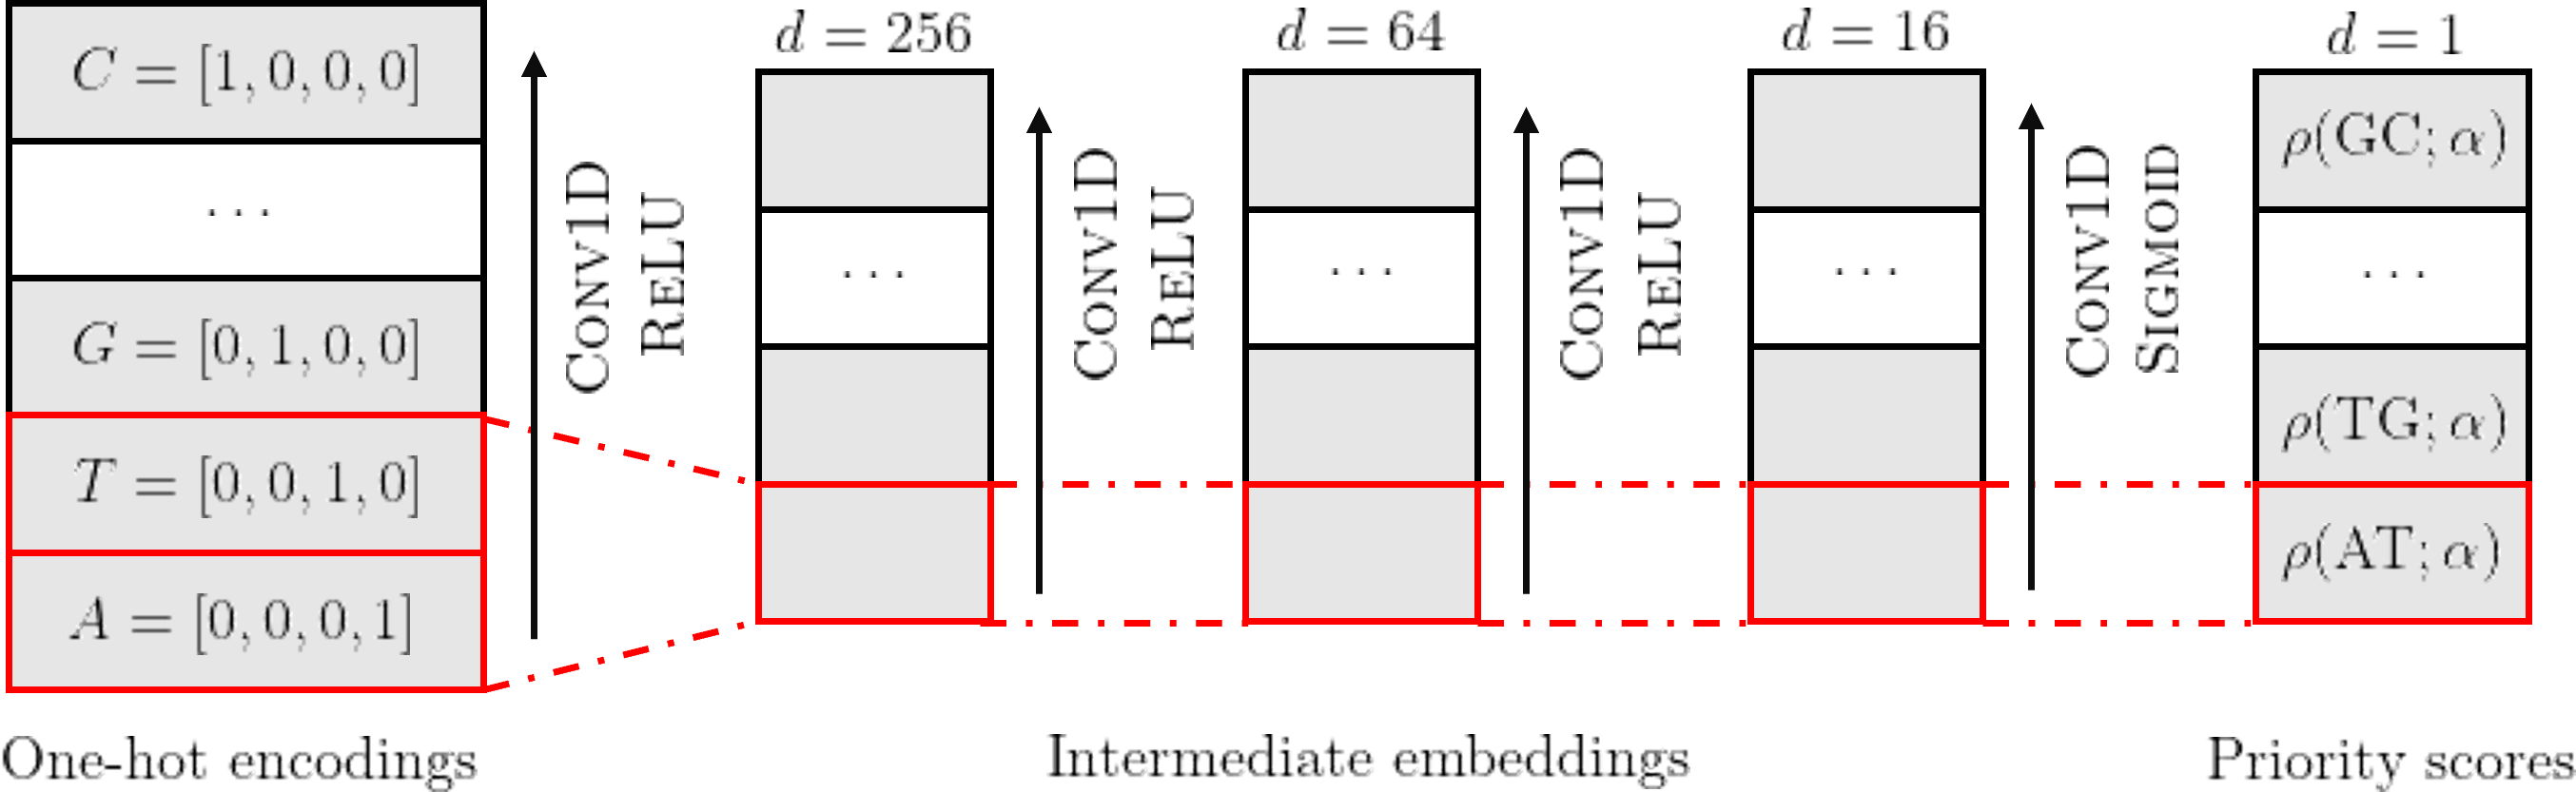
\includegraphics[width=0.95\columnwidth]{minimizer_plots/Priority Net Architecture.png} 
\end{tabular}
\caption{Our \textsc{PriorityNet} architecture for $k=2$, parameterized by weights $\alpha$, maps sequence multi-hot encoding to priority scores through a series of 3 convolution layers with kernel size $[k, 1, 1]$ and $[256, 64, 16]$ embedding channels respectively. Fixing network weights $\alpha$, the computation of any $k$-mer priority score is deterministic given its multi-hot encodings.}
\label{app-msd-fig:prioritynet}
\end{figure}

\subsection{Proxy Objective}
\label{c5-sec:objective}
The density computation in Eq.~\ref{eq:dual}, however, is not differentiable with respect to the network weights. As such, $\alpha$ cannot be readily optimized with established gradient back-propagation techniques used in most deep learning methods. To work around this, we introduce a proxy optimization objective that approximates Eq.~\ref{eq:dual} via coupling \textsc{PriorityNet} with another function called \textsc{TemplateNet}. Unlike the former, \textsc{TemplateNet} relaxes the \textit{consistency} requirement and generates \textit{template} score assignments that might not correspond to valid minimizer schemes. In exchange, such \textit{templates} are guaranteed to yield low densities by design.

Intuitively, the goals of these networks are complementary: \textsc{PriorityNet} generates valid minimizer schemes in the form of \textit{consistent} priority score assignments, whereas \textsc{TemplateNet} pinpoints neighborhoods of low-density score assignments situated around its output templates. This reveals an alternative optimization route where these networks negotiate towards a consensus solution that (a) satisfies the constraint enforced by \textsc{PriorityNet}; and (b) resembles a template in the output space of \textsc{TemplateNet}, thus potentially yielding low density. Let $f$ and $g$ denote our proposed \textsc{PriorityNet} and \textsc{TemplateNet}, respectively parameterized by weights $\alpha$ and ${\beta}$. Here $g$ is an atomic function that maps a $k$-mer index to a real-valued score in $[0, 1]$, and we also denote the output of applying $g$ on every $k$-mer indices as $\mathbf{g}(S;\beta)$. Last, we formalize our objective as minimizing a distance metric $\Delta$ between $\mathbf{f}$ and $\mathbf{g}$:
\begin{eqnarray}
(\alpha_\ast, \beta_\ast) &=& \underset{\alpha,\beta}{\mathrm{argmin}} \ \Delta\left(\mathbf{f}(S;\alpha),\mathbf{g}(S;{\beta})\right) \ .
\label{eq:proxy}
\end{eqnarray}  
We subsequently detail the full specification of our proxy objective, which includes two other components. First, Section~\ref{c5-sec:template} discusses the parameterization of our \textsc{TemplateNet} to consistently generate templates that achieve the theoretical lower-bound density~\citep{marcais17} on the target sequence. Section~\ref{c5-sec:divergence} then discusses a practical choice of $\Delta$ to accurately capture high-performing neighborhoods of minimizers. These specifications have strong implications on the expressiveness of the solution space and directly influences the performance of our framework, as shown in Section~\ref{c5-sec:exp}.


\subsection{Specification of TemplateNet}
\label{c5-sec:template}
The well-known theoretical lower bound $1/w$ for density implies that the optimal minimizer, if it exists, samples $k$-mers exactly $w$ positions~\citep{marcais17}. As a result, we will construct $g$ such that $\mathbf{g}(S;\beta)$ approximates this uniform assignment pattern given any initialization of its parameter $\beta$. Proposition~\ref{c5-lem:periodic} below shows a sufficient construction of $g$ such that $\mathbf{g}(S; \beta)$ approximately yields the optimal density.

\begin{proposition}
\label{c5-lem:periodic}
Let $g:\mathbb{R}\rightarrow[0,1]$ be a periodic function, with fundamental period $w$, such that $g$ has a unique minimum value on every $w$-long interval. Formally, $h$ satisfies:
\begin{eqnarray}
(1): \forall t \in \mathbb{R}: g(t) = g(t + w) \quad &\text{and}& \quad (2): \forall i, j \in \underset{t}{\mathrm{arginf}} \ h(t), \ \exists u \in \mathbb{N}: |i - j| = uw \nonumber \ .
\end{eqnarray}
Then, the template $\mathbf{g}(S; \beta) \triangleq [g(i)]_{i \in [L]}$ induces a sketch with density factor $1/w + o(1)$ on $S$ when $S$ is sufficiently long (i.e., $L_w \gg w^2$). 
\end{proposition} 
\begin{proof} 
We will now express the density of $S$ in terms of the template score assignment $g(S)$. Note that even though $g$ may not satisfy the consistency constraint, it will still induce a $k$-mer sampling scheme. Let $m(\kappa^{w_k}_t) \triangleq \underset{j\in[t, t+w]}{\mathrm{argmin}} \ g(j)$ be the selector function induced by $g$ of window $\kappa^{w_k}_t$, and let $\gamma_t$ indicates the event that the $t$-th window picks a different $k$-mer than the $(t-1)$-th window. Particularly, $\gamma_1 \triangleq 1$ and $\gamma_t \triangleq \mathbb{I}(m(\kappa^{w_k}_t) \neq m(\kappa^{w_k}_{t-1}))$. Then, the density of the scheme induced by $g(S)$ is given by:
\begin{eqnarray}
D(S; g)  &=& \frac{1}{L_w} \sum_{t=1}^{L_w}\gamma_t \ .
\end{eqnarray}
For any value of $u \in \mathbb{N}^{+}$, we further define the integer interval $\mathcal{I}_u \triangleq [(u-1)w + 1, uw]$. As the density of the entire sequence is simply the sum of density for each interval $\mathcal{I}_u$, it is then sufficient to derive the values of $\gamma_t$ for all values of $t$ in some arbitrary interval $\mathcal{I}_u$. 

Without loss of generality, we assume $0 \in \underset{t}{\mathrm{arginf}}\ g(t)$ since this can always be achieved via adding a constant phase shift to $g$. As $g$ has a period of $w$, this implies $\{uw \mid u \in \mathbb{N}^{+}\} \subseteq \underset{t}{\mathrm{arginf}}\ g(t)$, which further reduces to $\{uw \mid u \in \mathbb{N}^{+}\} \equiv \underset{t}{\mathrm{arginf}}\ g(t)$ when condition (2) holds. Then, it follows that $\forall t \neq uw$, we have $t \notin \underset{t}{\mathrm{arginf}}\ g(t)$. In addition, the index $uw$ is in the window $\kappa^{w_k}_{t}$ by definition. Together, the above facts imply that $\forall t: m(\kappa^{w_k}_{t}) = uw$ and consequently $\gamma_t = 0$ for all $t \neq (u-1)w + 1$, since the index $uw$ is overlapped by $\kappa^{w_k}_{(u-1)w + 1}$. For $u = 1$, we trivially have $\gamma_{(u-1)w + 1} = \gamma_1 = 1$ by definition. For any $u > 1$, we have $m(\kappa^{w_k}_{(u-1)w}) = (u-1)w$ and $m(\kappa^{w_k}_{(u-1)w + 1}) = uw$, which imply that $\gamma_{(u-1)w + 1} = 1$. Finally, using the above derivations, we have:
\begin{eqnarray}
\mathcal{D}(S; g) = \frac{1}{L_w}\left(c + \sum_{u=1}^{\lfloor\frac{L_w}{w}\rfloor}\sum_{t \in \mathcal{I}_u} \gamma_{t}  \right) =  \frac{1}{L_w}\left(c + \left\lfloor\frac{L_w}{w}\right\rfloor\right) \ ,
\end{eqnarray} 
where $c \triangleq \sum_{t=\lfloor\frac{L_w}{w}\rfloor w + 1}^{L_w} \gamma_t$ is the remainder of the sequence that does not make up any complete interval. The second equality follows from the derived values of $\gamma_t$ for $t \in \mathcal{I}_u$. Finally, using the fact that $c = L_w - \lfloor\frac{L_w}{w}\rfloor w< w$ and the sufficient length assumption $L_w \gg w^2$, we have:
\begin{eqnarray}
\frac{1}{L_w}\left(c + \left\lfloor\frac{L_w}{w}\right\rfloor\right) & < &  \frac{1}{w} + \frac{w}{L_w} \ \ = \ \ \frac{1}{w} + o(1) \ ,
\end{eqnarray} 
which concludes our proof.
\end{proof}

Note that the resulting sketch induced by $g$ does not necessarily correspond to a valid minimizer. While this sketch has guaranteed low density, it does not preserve the sequence identity like a minimizer sketch, hence is not useful for downstream applications. However, it is sufficient as a guiding template to help $\textsc{PriorityNet}$ navigating the space of orderings. By Proposition~\ref{c5-lem:periodic}, \textsc{TemplateNet} can be as simple as $g(t) = \sin(2\pi t/w)$ to induce a near-optimal score assignment. This na\"ive specification, however, encodes exactly a single set of template minima (i.e., one that picks $k$-mers from the set of interval positions $\{w, 2w, \dots\}$), which might not be in proximity of any valid minimizer scheme. For example, consider a sequence $S$ in which some particular $k$-mer uniquely occurs at positions $t \in \left\{\frac{1}{2}w, \frac{3}{2}w, \dots\right\}$. The ideal assignment would be such that minima will occur at these locations, which is impossible. 

It is therefore necessary that the specification of \textsc{TemplateNet} is sufficiently expressive for Eq.~\ref{eq:proxy} to find an optimal solution. To model this family of template functions, we subsequently propose several parameterization strategies using (1) an ensemble of sinusoidal functions with integer phase shifts or (2) a Fourier series model that encodes any arbitrary sinusoidal function. We further propose an independent positional phase-delay component that can be combined with (1) and (2) to encode template functions with approximately constant period.

\subsubsection{Ensemble Template Model}
\label{sec:ensemble}
We first give a construction of a periodic model such that every $k$-mer position appears in at least one template encoded by its parameter space. To achieve this, we employ a linear combination of multiple sine functions with fixed integer phase shifts  $\phi \in [w-1]$, each of which encodes a set of minima with a unique positional offset such as $\mathcal{T}_1=\{0, w, 2w, \dots\}, \mathcal{T}_2=\{1, w+1, 2w+1, \dots\}, \dots \ \mathcal{T}_{w-1}=\{w-1, 2w-1, 3w-1, \dots \}$. In particular, we define:
\begin{eqnarray}
g(t; \beta) &\triangleq& \sigma\left(\sum_{\phi=0}^{w-1} \beta_{\phi}\sin\left(\frac{2\pi}{w}(t + \phi)\right) \right) \ ,
\end{eqnarray}
where the sigmoid activation function $\sigma$ ensures that $h(t)$ appropriately maps to $[0, 1]$ and outputs scores on the same scale as $\textsc{PriorityNet}$; $\beta = \{\beta_{\phi}\}_{\phi=0}^{w-1}$ are optimizable amplitude parameters such that $\beta_\phi \geq 0$ and  $\sum_{\phi=1}^w\beta_{\phi} = 1$. Optimizing $\beta$ then determines the dominant phase shift $\phi_{\mathrm{max}} = \mathrm{argmax}_{\phi}\ \beta_{\phi}$, which in turn controls the final offset of the template minima. Additionally, allowing the amplitudes of the ensemble components to be optimizable also helps to generate sufficient slack room for matching the template scores against the priority scores.
\subsubsection{Truncated Fourier Series Template Model}
\label{sec:fourier}
The periodic function $g(t)$ with period $w$ can be generalized using a Fourier series, which is a linear combination of an infinite number of sine and cosine functions, whose frequencies are integer multiples of $1/w$:
\begin{eqnarray}
g(t; \beta) &=& \sigma\left(\beta_0 + \sum_{r=1}^\infty \left[ \beta_{r,1}\sin\left(\frac{2r\pi}{w}t\right) + \beta_{r,2}\cos\left(\frac{2r\pi}{w}t\right)\right]\right) \ ,
\end{eqnarray}
where $\beta = \{\beta_{r,1}, \beta_{r,2}\}_{r=0}^{\infty} \cup \{\beta_0\}$ are optimizable amplitude parameters. For computational efficiency, we approximate $g$ by a finite truncation up to the first $R$ summands of the above Fourier series:
\begin{eqnarray}
g(t; \beta) &\simeq& \sigma\left(\beta_0 + \sum_{r=1}^R \left[ \beta_{r,1}\sin\left(\frac{2r\pi}{w}t\right) + \beta_{r,2}\cos\left(\frac{2r\pi}{w}t\right)\right]\right) \ .\ 
\end{eqnarray}
Similar to the ensemble template model, optimizing the amplitude parameters $\beta$ of this model also determines the offset of the minima locations and adds slack room to help matching against the priority score assignment. 
\noindent The key difference between these two template models is that the ensemble model requires all $w$ phase shifts (and hence, all $w$ component functions) to encode every $k$-mer location, whereas the Fourier model can achieve the same with a fixed value of $R$ and remains compact even for large $w$. The Fourier model, however, will admit periodic functions whose minima do not coincide with integer indices, therefore condition (2) above will be less likely to hold in practice.

\subsubsection{Positional Phase-Shift Model}
\label{sec:phase}
By Proposition~\ref{c5-lem:periodic}, all template score assignments encoded by the above $\beta$-parameterized families of functions correspond to near-optimal minimizer schemes with approximately perfect density factors. However, we note that this set of template solutions is usually unrealistic and cannot be mirrored exactly by \textsc{PriorityNet}, especially on complex problem instances with more difficult scoring constraints. For example, while the theoretical lower bound for densityis $1/w$, the actual optimal density factor attainable given a specific sequence is often considerably larger and occurs when consecutive minimizer locations are not always exactly $w$ locations apart.

Motivated by this observation, we further extend our template model with a learnable component that adaptively adjusts the local frequencies of every encoded periodic function through adding positional noise to their phase shift parameters. That is, let $\xi(S; \gamma) \in [-1, 1]^L$ be a noise generating function parameterized by $\gamma$ and let $\xi_i(S; \gamma)$ be the noise value corresponding to the $i^{\text{th}}$ $k$-mer. We define the $(\epsilon, \gamma)$-augmented \textsc{TemplateNet} as:
\begin{eqnarray}
\mathbf{g}(S; \beta, \gamma) &\triangleq& \left[g\left(i + \epsilon \cdot \xi_i(S; \gamma); \beta\right)\right]_{i \in [l]} \ ,
\end{eqnarray}
where $\xi_i(S;\gamma)$ denotes the $i$-th entry of the noise vector. This will allow every entry in the template score assignment to be adjusted by a phase shift of up to $\epsilon$ in magnitude. When $\epsilon = 0$, this space of template functions coincides with that of the exact periodic template model, thus encodes all theoretical optimal assignments. On the other hand, as $\epsilon$ increases, more template assignments are admitted, but the optimal density guarantee becomes less certain.

\subsection{Specification of Distance Metric}
\label{c5-sec:divergence}
As standard practice, we first consider as our objective the $\ell^2$ distance, which is given by:
\begin{eqnarray}
\Delta_{\ell^2}(\mathbf{f}(S;\alpha), \mathbf{g}(S;\beta)) &\triangleq& \sum_{i=1}^{l} (\mathbf{f}_i(S;\alpha) - \mathbf{g}_i(S;\beta))^2 \ ,
\end{eqnarray}
where $\mathbf{f}_i$ and $\mathbf{g}_i$ are respectively the shorthands for the $i^{\text{th}}$ entries of $\mathbf{f}(S; \alpha)$ and $\mathbf{g}(S; \beta)$. For ease of notation, we assume that the notation $\beta$ also incorporate $\gamma$ in case the positional noise model is used. This metric, however, places an excessively strict matching objective at all locations along $\mathbf{f}$ and $\mathbf{g}$, which is often unnecessary. Indeed, it is sufficient to ensure that the $k$-mers at the selected locations are assigned lowest scores. Enforcing a perfect matching will take away the degrees of freedom needed for the proxy objective to satisfy the constraints implied by \textsc{PriorityNet} (i.e., a $k$-mer has to be assigned the same score at all of its occurrences). 

As such, we are interested in constructing an alternative distance metric that: (a) prioritizes matching $\mathbf{f}$ and $\mathbf{g}$ around the neighborhoods of minima; and (b) allows flexible assignment at other positions to admit more solutions that meet the consistency requirement. To accomplish these design goals, we propose the following asymmetrical distance metric:
\begin{eqnarray}
\Delta_{\mathcal{DM}}(\mathbf{f}(S; \alpha),\mathbf{g}(S; \beta)) &\triangleq& \sum_{i=1}^{L} \Big[(1  - \mathbf{g}_i) \cdot (\mathbf{f}_i - \mathbf{g}_i)^2 + \lambda \cdot(1-\mathbf{f}_i)^2 \Big] \ .
\label{eq:divfunc}
\end{eqnarray}
Specifically, the intuition behind the first component $(1 - \mathbf{g}_i) \cdot (\mathbf{f}_i - \mathbf{g}_i)^2$ in the summation is to weight each position-wise matching term $(\mathbf{f}_i - \mathbf{g}_i)^2$ by its corresponding template score. The weight term $1 - \mathbf{g}_i$ implies stronger matching preference around the minima of $\mathbf{g}$ where the template scores $\mathbf{g}_i$ are low; and vice-versa weaker matching preference at other locations where $\mathbf{g}_i$ are high. The second component $\lambda\cdot(1-\mathbf{f}_i)^2$, on the other hand, encourages \textsc{PriorityNet} to maximize its output scores whenever possible, which prevents the system from settling for a trivial solution where both $\mathbf{f}$ and $\mathbf{g}$ are squashed to zero. The trade-off between these two components is controlled by the magnitude of the hyper-parameter $\lambda$. Finally, we confirm that this distance metric is fully differentiable with respect to $\alpha, \beta$, hence can be efficiently optimized using gradient-based techniques. The parameter gradients are given by:
\begin{eqnarray}
\frac{\partial}{\partial \alpha} \Delta_{\mathcal{DM}}(\mathbf{f,g}) &=& \sum_{i=1}^l a_i \cdot \frac{\partial}{\partial \alpha}\mathbf{f}_i \ , \nonumber \\
\frac{\partial}{\partial \beta} \Delta_{\mathcal{DM}}(\mathbf{f,g}) &=& \sum_{i=1}^l b_i \cdot \frac{\partial}{\partial \beta}\mathbf{g}_i \ ,
\end{eqnarray} 
where the respective constants are derived as follows:
\begin{eqnarray}
a_i &=& 2\cdot(1-\mathbf{g}_i)\cdot(\mathbf{f}_i - \mathbf{g}_i) + 2\lambda\cdot(\mathbf{f}_i - 1) \ , \nonumber \\
b_i &=& -2\cdot (1-\mathbf{g}_i)\cdot(\mathbf{f}_i - \mathbf{g}_i) - (\mathbf{f}_i - \mathbf{g}_i)^2 \ .
\end{eqnarray}
\section{Experiments}
\label{c5-sec:exp}
We implement our method using PyTorch and deploy all experiments on a RTX-2060 GPU. Similar to many other deep learning workflows, each training epoch computes a batch loss which averages over $N = 10$ randomly sampled subsequences of length $l = 500 \times (w + k)$. We set $\lambda = 1$ and use architectures of \textsc{PriorityNet} and \textsc{TemplateNet} as given in Fig.~\ref{app-msd-fig:prioritynet} and Section~\ref{c5-sec:template} respectively. Network weights are optimized using the ADAM optimizer~\citep{kingma14adam} with learning rate $\eta = 5e^{-3}$. 

\subsection{Comparison baselines} We compare \textsc{DeepMinimizer} with the following benchmarks: (a)~random minimizer baseline; (b)~Miniception~\citep{zheng20miniception}; (c)~PASHA~\citep{ekim20pasha}; and (d)~PolarSet Minimizer~\citep{zheng21}. Among these methods, (d) is a sequence-specific minimizer scheme. For each method, we measure the density factor $\mathcal{D}(S;\cdot) \triangleq (w+1)D(S;\cdot)$ to align with the convention of previous work (i.e., the theoretical lower bound on density factor is thus $\mathcal{D}(S;\cdot) \geq 1 + 1/w$). Our empirical result is obtained on different segments of the human reference genome: (a) chromosome 1 (\textsc{Chr1}); (b) chromosome X (\textsc{ChrX}); (c) the centromere region of chromosome X~\citep{miga19} (which we denote by \textsc{ChrXC}); and (d) the full genome (\textsc{Hg38}). We used lexicographic ordering for PASHA as suggested by~\citet{zheng20miniception}. Random ordering is used to rank $k$-mers within the UHS for Miniception, and outside the layered sets for PolarSet. In most settings, we employ the Ensemble template model (Section~\ref{sec:ensemble}) with no positional phase-shift component (Section~\ref{sec:phase}) for \textsc{DeepMinimizer}. However, for scenarios with large $w$ values, we demonstrate that the Fourier template model with positional phase-shift is able to achieve better performance (Section~\ref{sec:compare_template})

\subsection{Visualizing the mechanism of \textsc{DeepMinimizer}} 
\begin{figure}[h]
\begin{tabular}{cc}
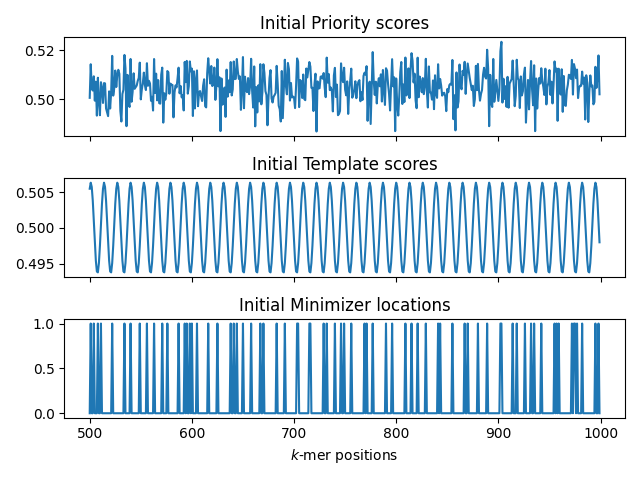
\includegraphics[width=0.47\columnwidth]{minimizer_plots/initial_visualize.png} & 
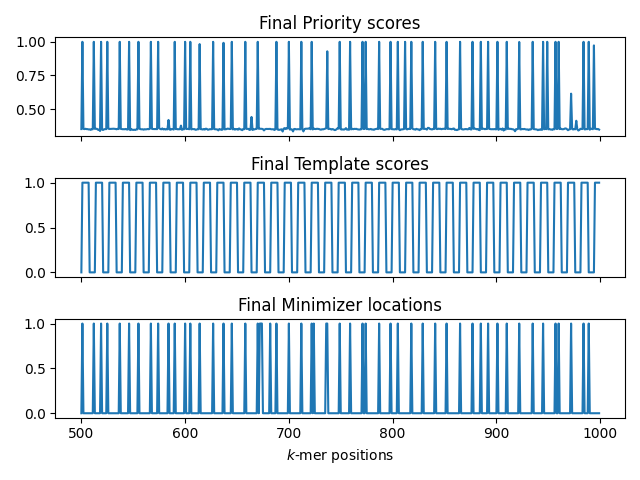
\includegraphics[width=0.47\columnwidth]{minimizer_plots/visualize.png}
\end{tabular}    
\caption{Visualization of \textsc{PriorityNet} and \textsc{TemplateNet} score assignments on positions $500-1000$ of \textsc{ChrXC} with $w=13$, $k=8$. Left: Initial assignments ($\mathcal{D}=2.05$); Right: Final assignments after $600$ training epochs ($\mathcal{D} = 1.39$). The bottom plots show corresponding locations of sampled $k$-mers: a value of $1$ means selected, and $0$ otherwise.}
\label{app-msd-fig:0}
\end{figure}

\noindent First, we show the transformation of the priority scores assigned by \textsc{ScoreNet} and \textsc{TemplateNet} over $600$ training epochs. Fig.~\ref{app-msd-fig:0} plots the outputs of these networks evaluated on positions $500$ to $1000$ of \textsc{ChrXC}, and their corresponding locations of sampled $k$-mers.

For ease of implementation, we employ the standard \textsc{MaxPool} operator from PyTorch to select window maxima as minimizer locations (instead of window minima, as previously formulated) . As a result, we expect the sampled locations in Fig.~\ref{app-msd-fig:0} to coincide with the peaks of the priority scores (instead of the troughs). We also note that to accommodate this implementation, every relevant term in the \textsc{DeepMinimizer} objective has been properly negated.

Initially, the \textsc{PriorityNet} assignment resembles that of a random minimizer and expectedly yields $\mathcal{D}=2.05$. After $600$ training epochs, the final \textsc{TemplateNet} assignment converges with a different phase shift than its initial assignment, but its period remains the same. Simultaneously, \textsc{PriorityNet} learns to match this template, hence induces a visibly sparser sketch with $\mathcal{D}=1.39$. This result demonstrates the negotiating behaviour of our twin architecture to find an optimal consensus score assignments.

\subsection{Convergence of our proxy objective} 
\begin{figure}[h]
\begin{tabular}{cc}
\includegraphics[width=0.46\columnwidth]{minimizer_plots/mznet_hg38_alL_w14.png} & 
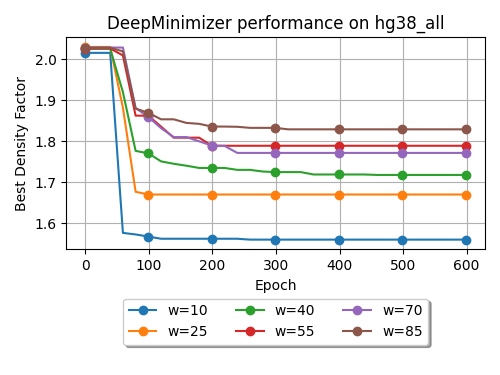
\includegraphics[width=0.46\columnwidth]{minimizer_plots/mznet_hg38_all_k13.png} 
\\
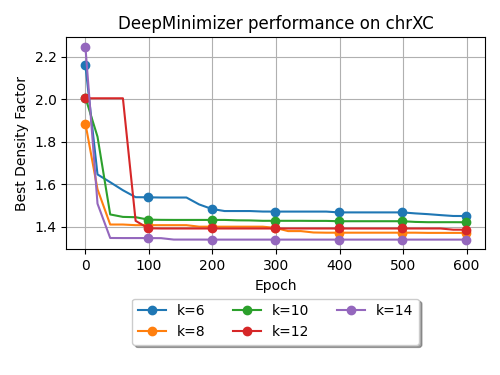
\includegraphics[width=0.46\columnwidth]{minimizer_plots/mznet_chrXC_w14.png} & 
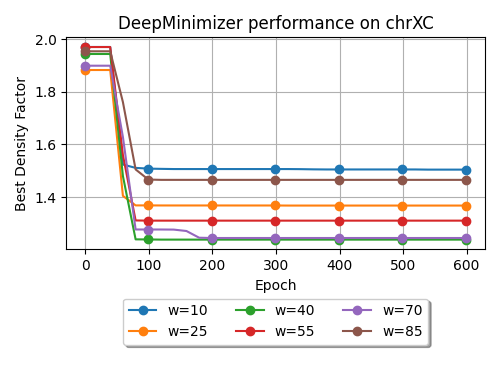
\includegraphics[width=0.46\columnwidth]{minimizer_plots/mznet_chrXC_k13.png}
\end{tabular}
\caption{Best density factors obtained by \textsc{DeepMinimizer} on \textsc{Hg38}, \textsc{ChrXC} over $600$ training epochs. Left: fix $w=13$, and vary $k \in \{6,8,10,12,14\}$; Right: fix $k=14$, and vary $w \in \{10, 25, 40, 55, 70, 85\}$.}
\label{app-msd-fig:1a}
\end{figure}

\noindent We further demonstrate that our proxy objective meaningfully improves minimizer performance as it is optimized. The first two columns of Fig.~\ref{app-msd-fig:1a} show the best density factors achieved by our method over $600$ epochs on two scenarios: (a) varying $k$ with fixed $w$; and (b) varying $w$ with fixed $k$. The experiment is repeated on \textsc{ChrXC} and \textsc{Hg38}. In every scenario, \textsc{DeepMinimizer} starts with $\mathcal{D}\simeq 2.0$, which is only comparable to a random minimizer. We observe steady decrease of $\mathcal{D}$ over the first $300$ epochs before reaching convergence, where total reduction ranges from $11-23\%$. 


Generally, larger $k$ values lead to better performance improvement at convergence. This is expected since longer $k$-mers are more likely to occur uniquely in the target sequence, which makes it easier for a minimizer to achieve sparse sampling. In fact, previous results have shown that when $k$ is much smaller than $\log w$, no minimizer will be able to achieve the theoretical lower-bound $\mathcal{D}$~\citep{zheng20miniception}. On the other hand, larger $w$ values lead to smaller improvements and generally slower convergence. This is because our ensemble parameterization of \textsc{TemplateNet} scales with the window size $w$ and becomes more complicated to optimize as $w$ increases. 

\subsection{Evaluating our proposed distance metric}  
\begin{figure}[h]
\begin{tabular}{cc}
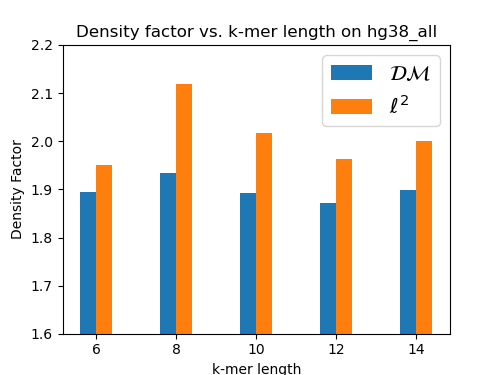
\includegraphics[width=0.46\columnwidth]{minimizer_plots/compare_divfunc_hg38_all.png} &
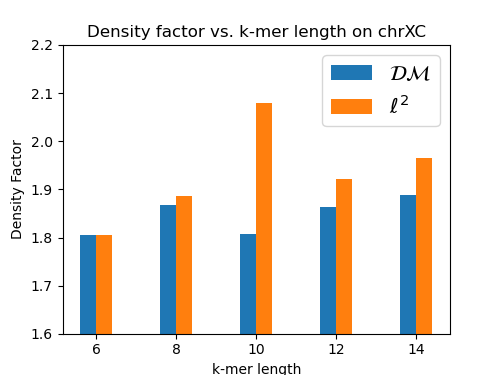
\includegraphics[width=0.46\columnwidth]{minimizer_plots/compare_divfunc_chrXC.png}
\end{tabular}    
\caption{Comparing best density factors obtained by \textsc{DeepMinimizer} with $\Delta_{\ell^2}$ and $\Delta_{\mathcal{DM}}$ on \textsc{Hg38} (left) and \textsc{ChrXC} (right) over $600$ training epochs.}
\label{app-msd-fig:1b}
\end{figure}

\noindent Fig.~\ref{app-msd-fig:1b} shows the density factors achieved by our \textsc{DeepMinimizer} method, respectively specified by the proposed distance metric $\Delta_{\mathcal{DM}}$ in Eq.~\ref{eq:divfunc} and $\Delta_{\ell^2}$ distance. Here, we fix $w=13$ and vary $k \in \{6,8,10,12,14\}$. We observe that with the $\Delta_{\ell^2}$ distance, we obtain performance similar to a random minimizer in most cases. On the other hand, with our divergence function, \textsc{DeepMinimizer} obtains significantly lower densities, which confirms the intuition in Section~\ref{c5-sec:divergence}.

\subsection{Comparing against other minimizer methods}
\begin{figure}[h]
\begin{tabular}{cc}
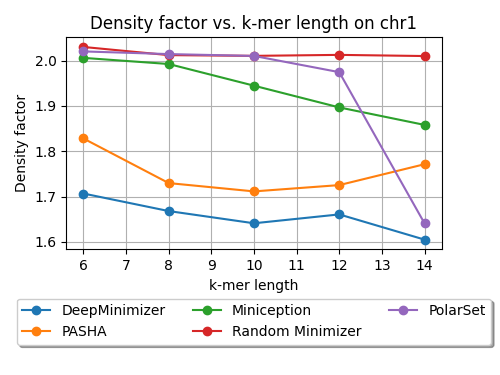
\includegraphics[width=0.46\columnwidth]{minimizer_plots/compare_k_chr1.png} & 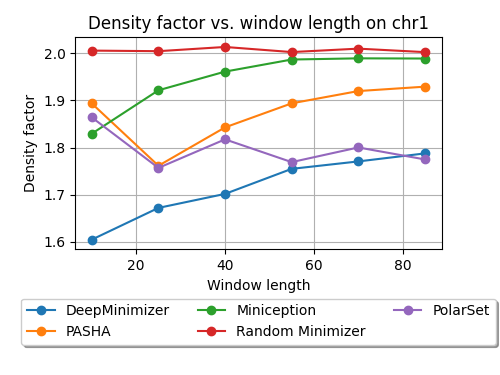
\includegraphics[width=0.46\columnwidth]{minimizer_plots/compare_w_chr1.png} \\
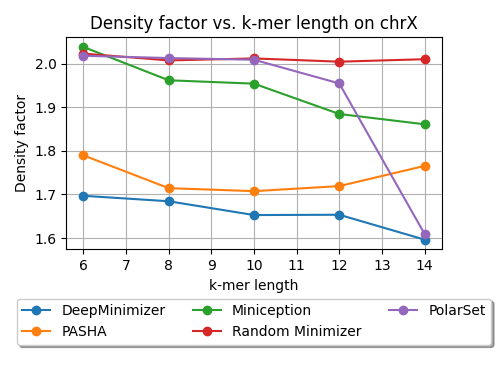
\includegraphics[width=0.46\columnwidth]{minimizer_plots/compare_k_chrX.png} & 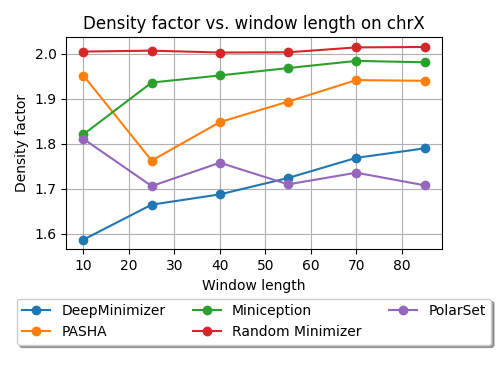
\includegraphics[width=0.46\columnwidth]{minimizer_plots/compare_w_chrX.png}
\end{tabular}
\caption{Density factors obtained by \textsc{DeepMinimizer} (600 training epochs), Random Minimizer, PASHA, Miniception and PolarSet on \textsc{Chr1}, \textsc{ChrX}. Left: fix $w=13$, and vary $k \in \{6,8,10,12,14\}$; Right: fix $k=14$, and vary $w \in \{10, 25, 40, 55, 70, 85\}$.}
\label{app-msd-fig:2a}
\end{figure}
\noindent We show the performance of \textsc{DeepMinimizer} compared to other benchmark methods. In this experiment, \textsc{DeepMinimizer} is trained for $600$ epochs with ensemble \textsc{TemplateNet} and no positional phase-shift. Fig.~\ref{app-msd-fig:2a} and Fig.~\ref{app-msd-fig:2b} shows the final density factors achieved by all methods, again on two comparison scenarios: (a) fix $w=13$, and vary $k \in \{6,8,10,12,14\}$; and (b) fix $k=14$, and vary $w \in \{10, 25, 40, 55, 70, 85\}$. 
\begin{figure}[h]
\begin{tabular}{cc}
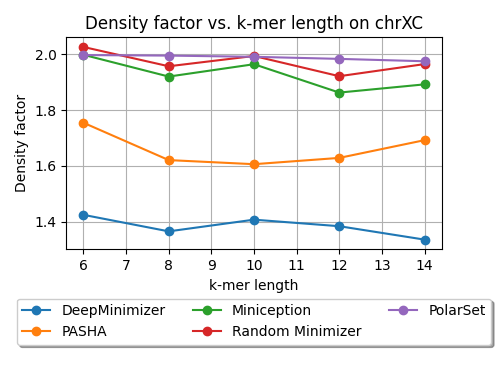
\includegraphics[width=0.46\columnwidth]{minimizer_plots/compare_k_chrXC.png} &
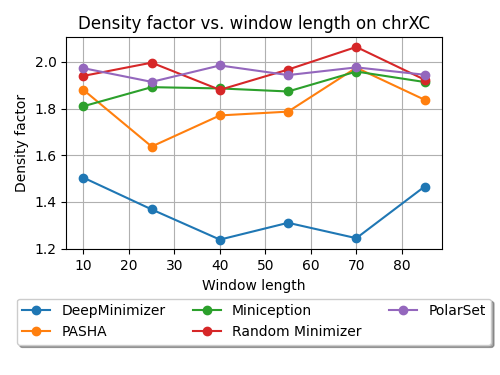
\includegraphics[width=0.46\columnwidth]{minimizer_plots/compare_w_chrXC.png} \\
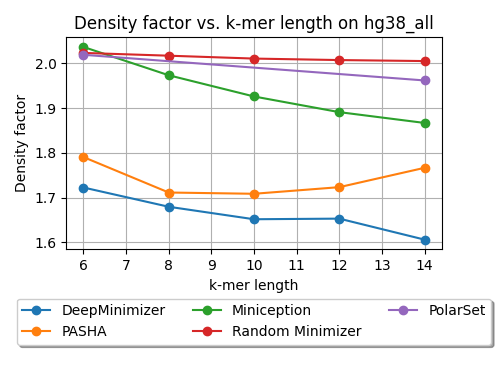
\includegraphics[width=0.46\columnwidth]{minimizer_plots/compare_k_hg38_all.png} &
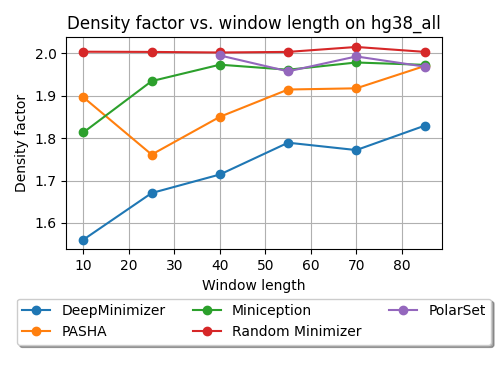
\includegraphics[width=0.46\columnwidth]{minimizer_plots/compare_w_hg38_all.png}
\end{tabular}    
\caption{Density factors obtained by \textsc{DeepMinimizer} (600 training epochs), Random Minimizer, PASHA, Miniception and PolarSet on \textsc{ChrXC}, \textsc{Hg38}. Left: fix $w=13$, and vary $k \in \{6,8,10,12,14\}$; Right: fix $k=14$, and vary $w \in \{10, 25, 40, 55, 70, 85\}$.}
\label{app-msd-fig:2b}
\end{figure}
\noindent \textsc{DeepMinimizer} consistently achieves better performance compared to \textit{non-sequence-specific} minimizers (i.e., PASHA, Miniception) on all settings. We observe up to $40\%$ reduction of density factor (e.g., on \textsc{ChrXC}, $w=70$, $k=14$), which clearly demonstrates the ability of \textsc{DeepMinimizer} to exploit \textit{sequence-specific} information. Furthermore, we also observe that \textsc{DeepMinimizer} outperforms our \textit{sequence-specific} competitor, PolarSet, in a majority of settings. The improvements over PolarSet are especially pronounced for smaller $k$ values, which are known harder tasks for minimizers~\citep{zheng20miniception}. On larger $w$ values, our method performs slightly worse than PolarSet in some settings. This is likely due to the added complexity of optimizing \textsc{TemplateNet}, as described in convergence ablation study of our method.

Notably, the centromere region of chromosome X (i.e., \textsc{ChrXC}) contains highly repetitive subsequences~\citep{fukagawa14} and has been shown to hamper performance of PolarSet~\citep{zheng21}. Fig.~\ref{app-msd-fig:2b} shows that PolarSet and the UHS-based methods perform similarly to a random minimizer, whereas our method is consistently better. Moreover, we observe that \textsc{DeepMinimizer} obtains near-optimal densities with \textsc{ChrXC} on several settings. For example, we achieved $\mathcal{D}=1.22$ when $k=14$, $w\in \{40,70\}$, which is significantly better than the results on \textsc{Chr1} and \textsc{ChrX}. This suggests that \textsc{ChrXC} is not necessarily more difficult to sketch, but rather good sketches have been excluded by the UHS and polar set reparameterizations, which is not the case with our framework.

\subsection{Number of unique k-mers in the final minimizer set}
\label{sec:compare_unique}
\begin{figure}[h]
\centering
\begin{tabular}{c}
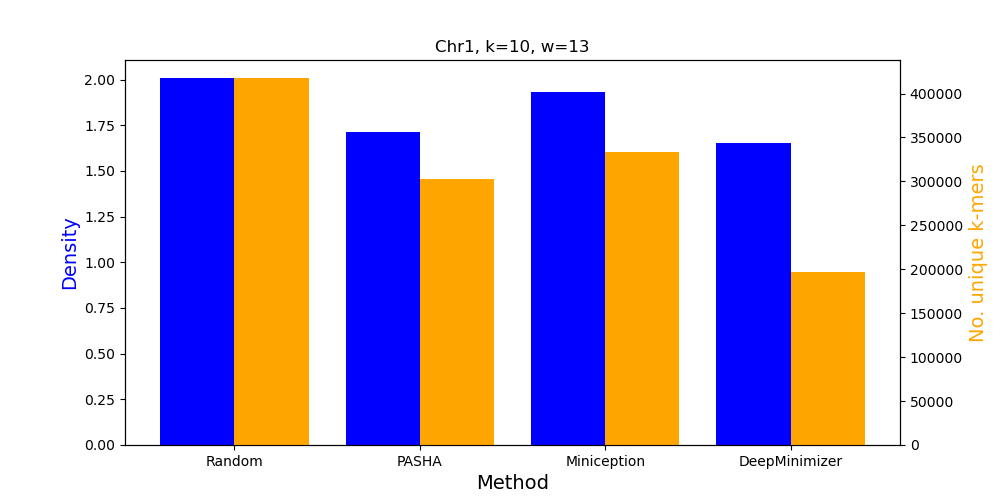
\includegraphics[width=0.96\columnwidth]{minimizer_plots/compare_unique_Chr1_w13_k10.png}
\end{tabular}
\caption{Comparing density and number of unique $k$-mers in the minimizer sets obtained by various benchmarks on \textsc{Chr1} with $k=10$ and $w=13$.}
\label{app-msd-fig:5a}
\end{figure}
\noindent This section investigates the numbers of unique $k$-mers in the final minimizer sets obtained by random ordering, PASHA, Miniception and DeepMinimizer. On Chromosome 1, with $k=10$ and $w=13$, Fig~\ref{app-msd-fig:5a} shows that the density factors and numbers of unique $k$-mers obtained by each method are strongly correlated. This agrees with the intuition of many other minimizer methods that a small set of high priority $k$-mers (e.g., a small UHS in the case of PASHA and Miniception) tends to induce a low density sketch on the target sequence. This observation is also expected since the $10$-mer distribution of \textsc{Chr1} is fairly similar to that of a random sequence, which aligns with the premise of most UHS-based minimizer theories. 
\begin{figure}[h]
\centering
\begin{tabular}{c}
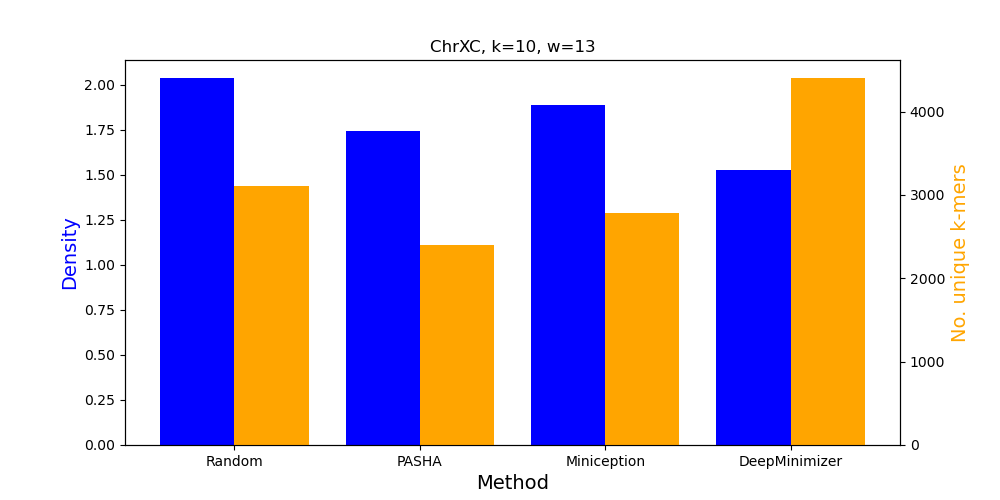
\includegraphics[width=0.96\columnwidth]{minimizer_plots/compare_unique_ChrXC_w13_k10.png} 
\end{tabular}
\caption{Comparing density and number of unique $k$-mers in the minimizer sets obtained by various benchmarks on \textsc{ChrXC} with $k=10$ and $w=13$.}
\label{app-msd-fig:5b}
\end{figure}

\noindent However, on the chromosome region of \textsc{ChrX}, which contains many highly repetitive sub-sequences, Fig.~\ref{app-msd-fig:5b} shows that in order to achieve the best density (i.e., $\mathcal{D}=1.526$), \textsc{DeepMinimizer} actually had to pick more high priority $k$-mers, not fewer. This interestingly demonstrates that minimizing the size of the UHS is not always a desirable surrogate objective on certain specific sequences, hence asserts the need for a robust sequence-specific optimizer. 

\subsection{Comparing template models on large window values}
\label{sec:compare_template}
\begin{figure}[h]
\centering
\begin{tabular}{cc}
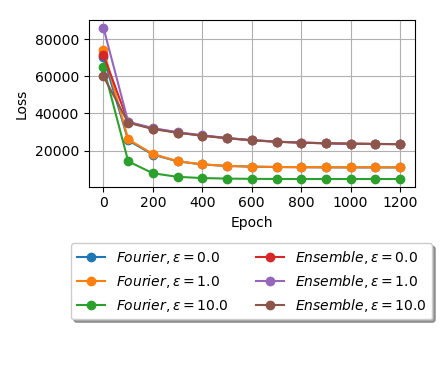
\includegraphics[width=0.46\columnwidth]{minimizer_plots/compare_template_loss.png} &
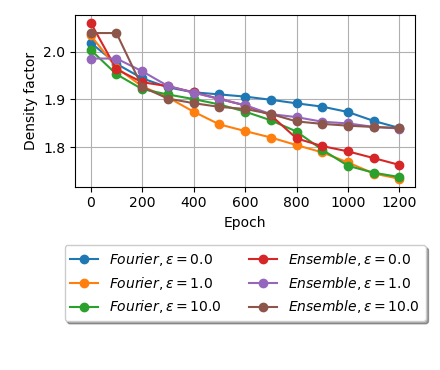
\includegraphics[width=0.46\columnwidth]{minimizer_plots/compare_template.png} 
\end{tabular}
\caption{Comparing loss (left) and best density obtained (right) over $1200$ training epochs on \textsc{Chr1} between ensemble and truncated Fourier series template models. Each template model is paired with a positional phase-shift component with $\epsilon\in\{0.0, 1.0, 10.0\}$.}
\label{app-msd-fig:6}
\end{figure}

\noindent In this section, we investigate the performance of \textsc{DeepMinimizer} on large window size with different template models. Particularly, we fixed $k=20, w=100$ and compare the best density factor obtained by \textsc{DeepMinimizer} over $1200$ training epochs  using the ensemble template model (Section~\ref{sec:ensemble}) and the truncated Fourier series template model (Section~\ref{sec:fourier}). We further pair each template model with a positional phase-shift component (Section~\ref{sec:phase}), with $\epsilon \in \{0.0, 1.0, 10.0\}$. We note that in each case, $\epsilon=0.0$ corresponds to the original template model. 

Fig.~\ref{app-msd-fig:6} shows the respective loss and density factor over $1200$ training epochs of these template models. First, we observe that in all models, the loss values correlate positively with the corresponding density factor. Generally, as the $\textsc{DeepMinimizer}$ loss decreases, the induced minimizer scheme also yields lower density factor on the input sequence, which suggests that our loss function is a good surrogate for the discrete density objective. 

Furthermore, we observe that among variants of the Fourier template model, both $\epsilon=1.0$ and $\epsilon=10.0$ perform significantly better than $\epsilon=0.0$. This is most likely because adding local phase perturbations indeed allows \textsc{TemplateNet} to encode more realistic near-optimal score assignments. In contrast, among variants of the ensemble template model, $\epsilon=0.0$ performs the best. This is most likely because the ensemble model has already accounted for all possible integer phase-shifts. As such, adding noisy phase perturbations with magnitude greater than $1.0$ will negatively affect the convergence of $\textsc{DeepMinimizer}$.

Finally, pairing Fourier template model with a positional phase-shift component of magnitude $\epsilon=1.0$ achieves the best performance out of all variants. This aligns with our intuition in Section~\ref{sec:fourier} regarding the trade-off between the certainty of Proposition~\ref{c5-lem:periodic} and the expressiveness of the admitted set of template score assignments.


\subsection{Runtime performance} Finally, we confirm that \textsc{DeepMinimizer} runs efficiently with GPU computing. In all of our experiments, each training epoch takes approximately $30$ seconds to $2$ minutes, depending on the choice of $k$ and $w$, which controls the batch size. Performance evaluation takes between several minutes (\textsc{ChrXC}) to $1$ hour (\textsc{Hg38}), depending on the length of the target sequence. Generally, our method is cost-efficient without frequent evaluations. Our most cost-intensive experiment (i.e., convergence ablation study on \textsc{Hg38}) requires a full-sequence evaluation every $20$ epochs over $600$ epochs, thus takes approximately $2$ days to complete. This is faster than PolarSet, which has a theoretical runtime of $\mathcal{O}(n^2)$ and takes several days to run with \textsc{Hg38}. We note that in real applications, we only have to evaluate once by the end of the training loop, which is much faster compared to PolarSet, whose running time above only involves building the minimizer scheme. 
\begin{figure}[h]
\centering
\begin{tabular}{cc}
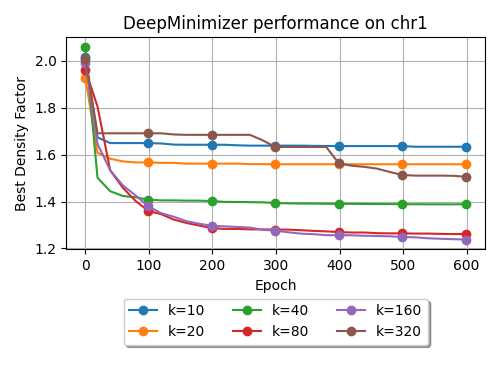
\includegraphics[width=0.45\columnwidth]{minimizer_plots/largek_chr1_w13.png} &
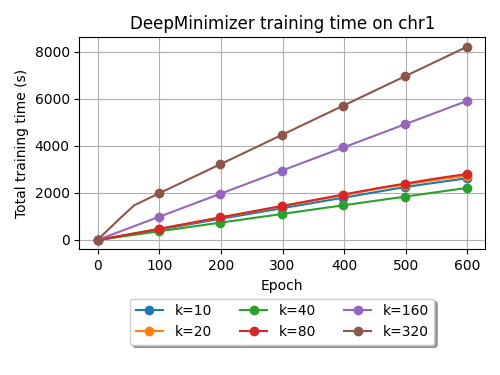
\includegraphics[width=0.45\columnwidth]{minimizer_plots/time_chr1_w13.png} 
\end{tabular}
\caption{Best density obtained (left) and runtime (right) of \textsc{DeepMinimizer} for $w=13$ and $k\in \{10, 20, 40, 80, 160, 320\}$ on \textsc{Chr1}.}
\label{app-msd-fig:7}
\end{figure}

\noindent Fig.~\ref{app-msd-fig:7} (right) measures runtime (in seconds) of \textsc{DeepMinimizer} on $\textsc{Chr1}$ over $600$ epochs. Larger $k$ values require \textsc{PriorityNet} to have more parameters. We expect running time for $k=40, 80, 160, 320$ to increase in the same order. For $k=10$ and $20$, however, the running times are approximately the same as $k=80$. We note that a smaller $k$ value means there are more $k$-mers in the same sequence. As such, even though \textsc{PriorityNet} is more compact for these values of $k$, we will incur some overhead from querying it more often. For completeness, we also show the corresponding density performance plot in Fig.~\ref{app-msd-fig:7} (left), which confirms that our model converges well even for large $k$.